\subsection{\textit{Type Ia} : Combination of the Buck/Boost Converter :}
The figure\ref{fig:Type 1a Active Battery Balancing} illustrates the Type Ia balancing method for a battery system with n series-connected cells. The description is stack-to-cells-to-stack in accordance with the accepted nomenclature. A buck converter serves as a charging unit that distributes charge from the stack to the chosen cells. A boost converter reverses the process of discharge.
\\
The boost converter's input and output voltage ranges must be large enough to accommodate cells with voltages ranging from 1 to n-1. All cells can be actively charged and discharged up to the top level of the stack in this manner. It is only possible for nearby cells to balance numerous cells at once. Access to all cells below the topmost cell is used to balance that cell.
\\
This section explains the balancing procedure shown in Figure \ref{fig:Type 1a Active Battery Balancing}. The buck converter feeds Cell 1 with energy from the stack through switch \textit{$S_wA1$}. The converter output current $I_{Buck}$ is used to charge Cell 1. With the converter input current boost, the boost converter simultaneously discharges Cell 1 and Cell 2 through \textit{$S_wB2$}. The sum of the current in Cell 1 is 0A since $I_{Buck} = -I_{Boost} = I_{Bal}$, while Cell 2 discharges with $I_{boost}$A (negative balancing or "discharge mode"). The buck converter is often connected higher than the boost converter Batteries in Charging Mode. Discharging is done in the opposite order.
\\

\begin{figure}[h]
	\centering
	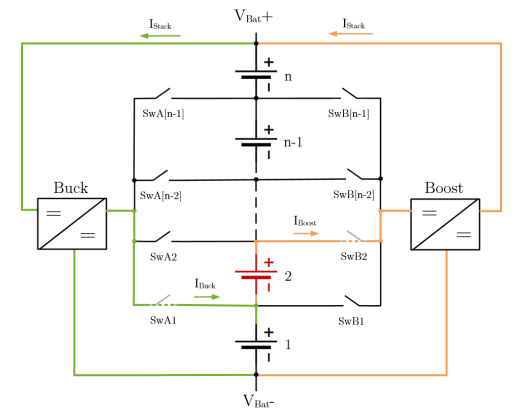
\includegraphics[width=0.7\textwidth]{Chap04/Figures/Type1a_ABMS.PNG}
	\caption{\textit{Type Ia}: Active Battery Balancing} 
	\label{fig:Type 1a Active Battery Balancing}
\end{figure}

The idle cell currents can be expressed as a vector following \ref{eq:Type1_cell_current}. It accounts for the balancing currents, both positive and negative, as well as the resulting stack current.
\begin{equation}\label{eq:Type1_cell_current}
    \vec{I_{Cell}}  = I_{stack} + \vec{I_n}\centerdot I_{Bal} - \vec{OUT}\centerdot I_{Bal}
\end{equation}

\begin{equation}\label{eq:Type1_cell_current}
    I_{stack}  = I_{Bal}(\frac{1}{\eta } \sum_{}^{}\vec{I_n}  ) + \vec{I_n}\centerdot I_{Bal} - \vec{OUT}\centerdot I_{Bal} \\
    \vec{I_n}  = \begin{pmatrix}
        S_{A1}\\
        \vdots
        S_{A[n-1]}
    \end{pmatrix} \\
    \vec{OUT}  = \begin{pmatrix}
        S_{B1}\\
        \vdots
        S_{B[n-1]} , S_{x}=\left\{0;1\right\} 
    \end{pmatrix} \\

\end{equation}